\documentclass{article}
\usepackage{fontspec}
\setsansfont{Helvetica}
\renewcommand{\familydefault}{\sfdefault}
\usepackage{tikz}
\usetikzlibrary{arrows.meta}
\pagestyle{empty}
\definecolor{cA}{HTML}{1F77B4}
\definecolor{cB}{HTML}{FF7F0E}
\definecolor{lookup}{HTML}{2A78D6}
\definecolor{lookuplight}{HTML}{9DC1EC}
\definecolor{write}{HTML}{EB6834}
\definecolor{writelight}{HTML}{F5B597}
\definecolor{ink}{HTML}{0B0B0B}
\definecolor{inktwo}{HTML}{52514E}
\definecolor{gridc}{HTML}{E4E3DF}
\definecolor{axisc}{HTML}{8F8E89}
\definecolor{refc}{HTML}{3D3C39}
\tikzset{
  tick/.style={font=\footnotesize, text=black, inner sep=1.5pt},
  lab/.style={font=\small, text=ink, inner sep=1.5pt},
  note/.style={font=\footnotesize, text=inktwo, inner sep=1.5pt},
  ser/.style={line width=1.4pt, line cap=round, line join=round},
  thin/.style={line width=0.9pt, line cap=round, line join=round},
  ref/.style={line width=0.8pt, draw=refc, dash pattern=on 3pt off 2pt},
}
\begin{document}
\setbox0=\hbox{%
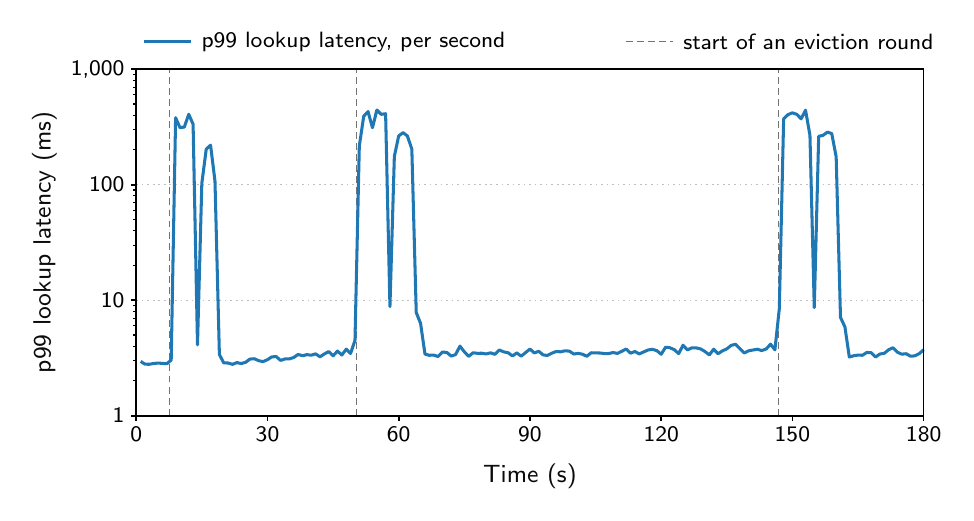
\begin{tikzpicture}[x=1cm,y=1cm]
\draw[black!25, line width=0.4pt, dash pattern=on 0.6pt off 1.4pt] (0.000,0.000) -- (10.000,0.000);
\draw[black, line width=0.6pt] (0.000,0.000) -- (-0.070,0.000);
\node[tick, anchor=east] at (-0.090,0.000) {1};
\draw[black!25, line width=0.4pt, dash pattern=on 0.6pt off 1.4pt] (0.000,1.467) -- (10.000,1.467);
\draw[black, line width=0.6pt] (0.000,1.467) -- (-0.070,1.467);
\node[tick, anchor=east] at (-0.090,1.467) {10};
\draw[black!25, line width=0.4pt, dash pattern=on 0.6pt off 1.4pt] (0.000,2.933) -- (10.000,2.933);
\draw[black, line width=0.6pt] (0.000,2.933) -- (-0.070,2.933);
\node[tick, anchor=east] at (-0.090,2.933) {100};
\draw[black!25, line width=0.4pt, dash pattern=on 0.6pt off 1.4pt] (0.000,4.400) -- (10.000,4.400);
\draw[black, line width=0.6pt] (0.000,4.400) -- (-0.070,4.400);
\node[tick, anchor=east] at (-0.090,4.400) {1,000};
\draw[black, line width=0.4pt] (0.000,0.442) -- (-0.040,0.442);
\draw[black, line width=0.4pt] (0.000,0.700) -- (-0.040,0.700);
\draw[black, line width=0.4pt] (0.000,0.883) -- (-0.040,0.883);
\draw[black, line width=0.4pt] (0.000,1.025) -- (-0.040,1.025);
\draw[black, line width=0.4pt] (0.000,1.141) -- (-0.040,1.141);
\draw[black, line width=0.4pt] (0.000,1.239) -- (-0.040,1.239);
\draw[black, line width=0.4pt] (0.000,1.325) -- (-0.040,1.325);
\draw[black, line width=0.4pt] (0.000,1.400) -- (-0.040,1.400);
\draw[black, line width=0.4pt] (0.000,1.908) -- (-0.040,1.908);
\draw[black, line width=0.4pt] (0.000,2.166) -- (-0.040,2.166);
\draw[black, line width=0.4pt] (0.000,2.350) -- (-0.040,2.350);
\draw[black, line width=0.4pt] (0.000,2.492) -- (-0.040,2.492);
\draw[black, line width=0.4pt] (0.000,2.608) -- (-0.040,2.608);
\draw[black, line width=0.4pt] (0.000,2.706) -- (-0.040,2.706);
\draw[black, line width=0.4pt] (0.000,2.791) -- (-0.040,2.791);
\draw[black, line width=0.4pt] (0.000,2.866) -- (-0.040,2.866);
\draw[black, line width=0.4pt] (0.000,3.375) -- (-0.040,3.375);
\draw[black, line width=0.4pt] (0.000,3.633) -- (-0.040,3.633);
\draw[black, line width=0.4pt] (0.000,3.816) -- (-0.040,3.816);
\draw[black, line width=0.4pt] (0.000,3.958) -- (-0.040,3.958);
\draw[black, line width=0.4pt] (0.000,4.075) -- (-0.040,4.075);
\draw[black, line width=0.4pt] (0.000,4.173) -- (-0.040,4.173);
\draw[black, line width=0.4pt] (0.000,4.258) -- (-0.040,4.258);
\draw[black, line width=0.4pt] (0.000,4.333) -- (-0.040,4.333);
\draw[black, line width=0.6pt] (0.000,0.000) -- (0.000,-0.070);
\node[tick, anchor=north] at (0.000,-0.090) {0};
\draw[black, line width=0.6pt] (1.667,0.000) -- (1.667,-0.070);
\node[tick, anchor=north] at (1.667,-0.090) {30};
\draw[black, line width=0.6pt] (3.333,0.000) -- (3.333,-0.070);
\node[tick, anchor=north] at (3.333,-0.090) {60};
\draw[black, line width=0.6pt] (5.000,0.000) -- (5.000,-0.070);
\node[tick, anchor=north] at (5.000,-0.090) {90};
\draw[black, line width=0.6pt] (6.667,0.000) -- (6.667,-0.070);
\node[tick, anchor=north] at (6.667,-0.090) {120};
\draw[black, line width=0.6pt] (8.333,0.000) -- (8.333,-0.070);
\node[tick, anchor=north] at (8.333,-0.090) {150};
\draw[black, line width=0.6pt] (10.000,0.000) -- (10.000,-0.070);
\node[tick, anchor=north] at (10.000,-0.090) {180};
\draw[black!55, line width=0.6pt, dash pattern=on 2.5pt off 1.5pt] (0.421,0.000) -- (0.421,4.400);
\draw[black!55, line width=0.6pt, dash pattern=on 2.5pt off 1.5pt] (2.796,0.000) -- (2.796,4.400);
\draw[black!55, line width=0.6pt, dash pattern=on 2.5pt off 1.5pt] (8.157,0.000) -- (8.157,4.400);
\draw[line width=1.1pt, line join=round, draw=cA] (0.056,0.689) -- (0.111,0.654) -- (0.167,0.653) -- (0.222,0.663) -- (0.278,0.668) -- (0.333,0.664) -- (0.389,0.660) -- (0.444,0.706) -- (0.500,3.784) -- (0.556,3.657) -- (0.611,3.666) -- (0.667,3.828) -- (0.722,3.701) -- (0.778,0.899) -- (0.833,2.951) -- (0.889,3.385) -- (0.944,3.436) -- (1.000,2.979) -- (1.056,0.777) -- (1.111,0.670) -- (1.167,0.669) -- (1.222,0.652) -- (1.278,0.674) -- (1.333,0.662) -- (1.389,0.678) -- (1.444,0.719) -- (1.500,0.723) -- (1.556,0.698) -- (1.611,0.687) -- (1.667,0.711) -- (1.722,0.747) -- (1.778,0.750) -- (1.833,0.702) -- (1.889,0.720) -- (1.944,0.721) -- (2.000,0.739) -- (2.056,0.778) -- (2.111,0.761) -- (2.167,0.775) -- (2.222,0.768) -- (2.278,0.785) -- (2.333,0.748) -- (2.389,0.784) -- (2.444,0.814) -- (2.500,0.760) -- (2.556,0.821) -- (2.611,0.770) -- (2.667,0.845) -- (2.722,0.790) -- (2.778,0.956) -- (2.833,3.425) -- (2.889,3.803) -- (2.944,3.862) -- (3.000,3.657) -- (3.056,3.882) -- (3.111,3.827) -- (3.167,3.835) -- (3.222,1.386) -- (3.278,3.293) -- (3.333,3.553) -- (3.389,3.594) -- (3.444,3.552) -- (3.500,3.385) -- (3.556,1.310) -- (3.611,1.172) -- (3.667,0.782) -- (3.722,0.767) -- (3.778,0.770) -- (3.833,0.751) -- (3.889,0.808) -- (3.944,0.803) -- (4.000,0.757) -- (4.056,0.776) -- (4.111,0.884) -- (4.167,0.811) -- (4.222,0.753) -- (4.278,0.799) -- (4.333,0.792) -- (4.389,0.793) -- (4.444,0.784) -- (4.500,0.798) -- (4.556,0.779) -- (4.611,0.834) -- (4.667,0.810) -- (4.722,0.800) -- (4.778,0.758) -- (4.833,0.797) -- (4.889,0.756) -- (4.944,0.801) -- (5.000,0.846) -- (5.056,0.797) -- (5.111,0.818) -- (5.167,0.772) -- (5.222,0.765) -- (5.278,0.794) -- (5.333,0.815) -- (5.389,0.811) -- (5.444,0.824) -- (5.500,0.820) -- (5.556,0.783) -- (5.611,0.791) -- (5.667,0.781) -- (5.722,0.754) -- (5.778,0.799) -- (5.833,0.797) -- (5.889,0.796) -- (5.944,0.789) -- (6.000,0.789) -- (6.056,0.802) -- (6.111,0.791) -- (6.167,0.818) -- (6.222,0.846) -- (6.278,0.794) -- (6.333,0.815) -- (6.389,0.784) -- (6.444,0.810) -- (6.500,0.834) -- (6.556,0.843) -- (6.611,0.826) -- (6.667,0.780) -- (6.722,0.869) -- (6.778,0.863) -- (6.833,0.838) -- (6.889,0.788) -- (6.944,0.895) -- (7.000,0.835) -- (7.056,0.862) -- (7.111,0.861) -- (7.167,0.848) -- (7.222,0.815) -- (7.278,0.772) -- (7.333,0.844) -- (7.389,0.787) -- (7.444,0.823) -- (7.500,0.848) -- (7.556,0.893) -- (7.611,0.907) -- (7.667,0.851) -- (7.722,0.796) -- (7.778,0.824) -- (7.833,0.834) -- (7.889,0.844) -- (7.944,0.827) -- (8.000,0.847) -- (8.056,0.908) -- (8.111,0.836) -- (8.167,1.359) -- (8.222,3.770) -- (8.278,3.824) -- (8.333,3.846) -- (8.389,3.827) -- (8.444,3.770) -- (8.500,3.880) -- (8.556,3.561) -- (8.611,1.372) -- (8.667,3.548) -- (8.722,3.560) -- (8.778,3.601) -- (8.833,3.583) -- (8.889,3.287) -- (8.944,1.248) -- (9.000,1.128) -- (9.056,0.745) -- (9.111,0.761) -- (9.167,0.770) -- (9.222,0.767) -- (9.278,0.803) -- (9.333,0.800) -- (9.389,0.745) -- (9.444,0.783) -- (9.500,0.792) -- (9.556,0.838) -- (9.611,0.863) -- (9.667,0.806) -- (9.722,0.781) -- (9.778,0.787) -- (9.833,0.755) -- (9.889,0.760) -- (9.944,0.788) -- (10.000,0.837);
\draw[black, line width=0.6pt] (0.000,0.000) rectangle (10.000,4.400);
\node[lab, anchor=north] at (5.000,-0.550) {Time (s)};
\node[lab, rotate=90, anchor=south] at (-0.950,2.200) {p99 lookup latency (ms)};
\draw[line width=1.1pt, line join=round, draw=cA] (0.100,4.750) -- (0.700,4.750);
\node[tick, anchor=west] at (0.770,4.750) {p99 lookup latency, per second};
\draw[black!55, line width=0.6pt, dash pattern=on 2.5pt off 1.5pt] (6.220,4.750) -- (6.820,4.750);
\node[tick, anchor=west] at (6.890,4.750) {start of an eviction round};
\end{tikzpicture}}%
\pdfvariable horigin=0pt
\pdfvariable vorigin=0pt
\pagewidth=\dimexpr\wd0+8pt\relax
\pageheight=\dimexpr\ht0+\dp0+8pt\relax
\shipout\vbox{\kern4pt\hbox{\kern4pt\box0\kern4pt}\kern4pt}
\end{document}
